\documentclass[letterpaper]{article}
\usepackage{natbib}
\usepackage[utf8]{inputenc}
\usepackage{graphicx}
\usepackage{color}
\usepackage{multirow}
\usepackage{amsmath}
\usepackage{array}
\usepackage{subcaption}
\usepackage{mathpazo}
\usepackage[a4paper]{geometry}

\title{Learning Dynamics: Assignment 2 \\
\Large Evolutionary dynamics in a spatial context}
\author{\Large Hakim Boulahya \\
hboulahy@ulb.ac.be\\
\\
Université Libre de Bruxelles
}

\begin{document}
\maketitle
\tableofcontents
\newpage

\section{Part I}

\paragraph{Specifications}
Plots in this part shows the average cooperation level of 100
simulations with unconditional imitation as the update mechanism.
The first rounds were played randomly,
where a player would choose cooperate with a probabilty of $\frac{1}{2}$.

\subsection{Neighborhood analysis}

\label{neighborpart1}
\paragraph{Remark} The analysis is based on results from 50x50 lattice
simulations.

\paragraph{Moore}

Figure \ref{fig:50moorepart1} shows the average cooperation level
using a Moore neighborhood for each player.
We can observe that the level after the first randomly played round, the
cooperation dropped at around 2\%. Then grows to stabilize at around 87\%.

\paragraph{Von Neumann}

Figure \ref{fig:50vonpart1} shows the average cooperation level
using a Von Neumann neighborhood for each player.
We can observe that the level after the first randomly played round, the
cooperation dropped at around 15\%. Then grows to stabilize at around 40\%.

\paragraph{}

We can see that the cooperation level follows the same pattern but on a
different scale. With Moore we have more neighbors, which can explain
why the behaviour of the players are more \textit{extreme}.

\subsection{Lattice observation}

Figure \ref{fig:visu50part1} shows the full matrix of cooperation for
the rounds $t_{0}, t_{1}, t_{5}, t_{10}, t_{20}, t_{50}$. We can observe
that in the first round there is more or less the same number of players
cooperating and defecting. But in the second round, a large percentage
of players will choose to defect, leaving only smalls zone of cooperation.
This is due to the fact that a defecting player will usually have a better
score around a mixed neighborhood of player than a cooperating player.
But when a cooperating player has a cooperating neighborhood he will have
high enough score to influence defecting players in his neighborhood. We can
observe that in the following rounds, a sort of \textit{cluster} of cooperation
will be formed and influence the full lattice until reaching the cooperation
level explained in section \ref{neighborpart1}.



\subsection{Lattice size analysis}

\paragraph{}

Figure \ref{fig:otherpart1}  shows the average cooperation level
of lattices of size 20, 12, 8 and 4. The behavior seems to the same
as in the analysis made against lattice of size 50
in section \ref{neighborpart1}, it crashes to a small level of cooperation
to grows and stabilize after a number of rounds. The plots show that when
the lattice size is small, the cooperation stabilize to a smaller cooperation
level than bigger lattices. We can observe that for a size 4 lattice,
the cooperation level is even 0 after the first round.

\paragraph{}

The reason could be that there is less players so less possibilities to
form some cooperation neighborhood, that will form the \texttt{clusters}
and grews as explained in previous section.

% Coop level for 50
\begin{figure}
    \begin{subfigure}{.5\textwidth}
        \centering
        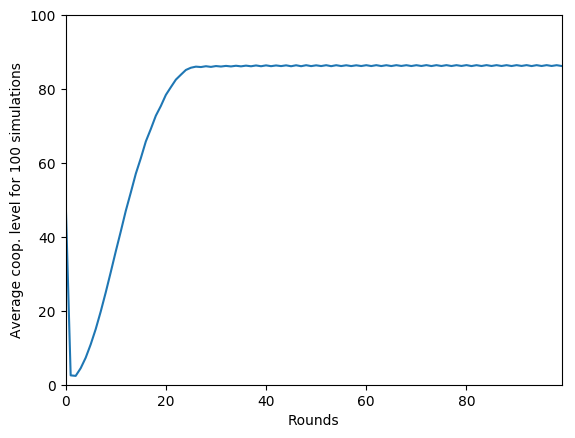
\includegraphics[width=1\linewidth]{images/assign2/50-part1}
        \caption{Moore neighborhood}
        \label{fig:50moorepart1}
    \end{subfigure}
    \begin{subfigure}{.5\textwidth}
        \centering
        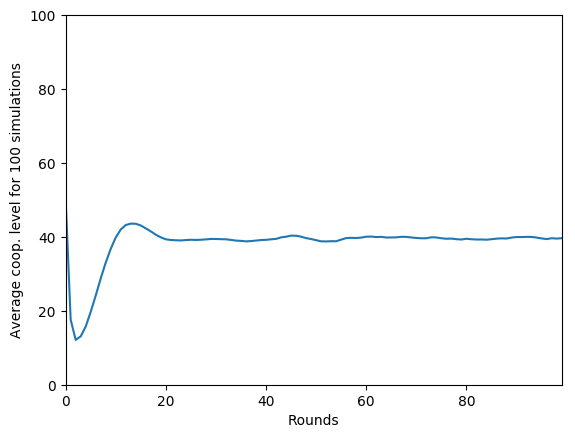
\includegraphics[width=1\linewidth]{images/assign2/50_vonneumann-part1}
        \caption{Von Neumann neigborhood}
        \label{fig:50vonpart1}
    \end{subfigure}
    \caption{Cooperation level using unconditional imitation and
    weak prisoner's dilemma on a 50x50 lattice}
    \label{fig:50part1}
\end{figure}

% Visualization for 50

\begin{figure}
    \begin{subfigure}{.33\textwidth}
      \centering
      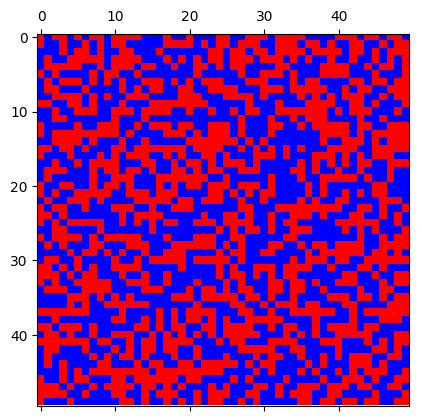
\includegraphics[width=1\linewidth]{images/assign2/visu_50-part1/t0}
      \caption{$t_0$}
      \label{fig:t0_50part1}
    \end{subfigure}
    \begin{subfigure}{.33\textwidth}
      \centering
      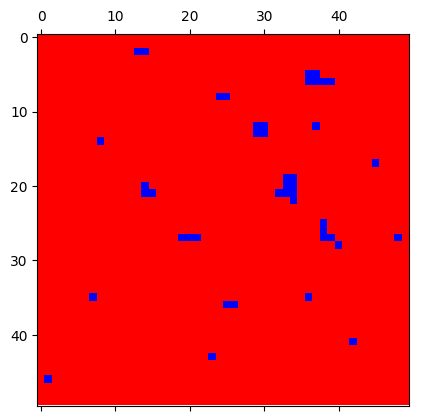
\includegraphics[width=1\linewidth]{images/assign2/visu_50-part1/t1}
      \caption{$t_1$}
      \label{fig:t1_50part1}
    \end{subfigure}
    \begin{subfigure}{.33\textwidth}
      \centering
      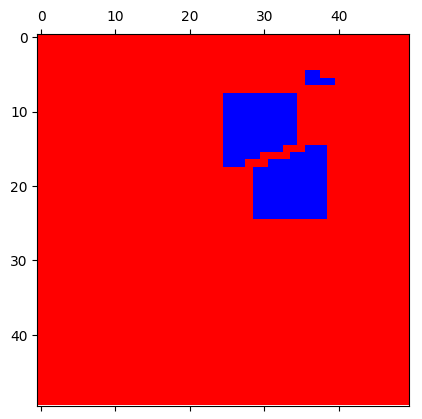
\includegraphics[width=1\linewidth]{images/assign2/visu_50-part1/t5}
      \caption{$t_5$}
      \label{fig:t5_50part1}
    \end{subfigure}
    \begin{subfigure}{.33\textwidth}
      \centering
      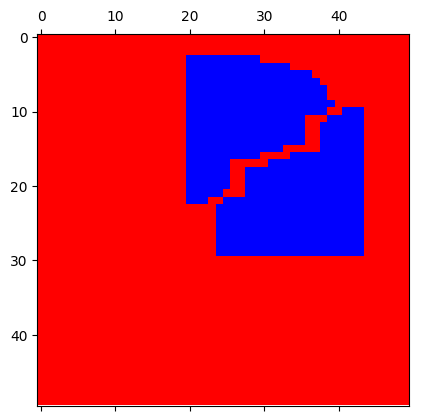
\includegraphics[width=1\linewidth]{images/assign2/visu_50-part1/t10}
      \caption{$t_{10}$}
      \label{fig:t10_50part1}
    \end{subfigure}
    \begin{subfigure}{.33\textwidth}
      \centering
      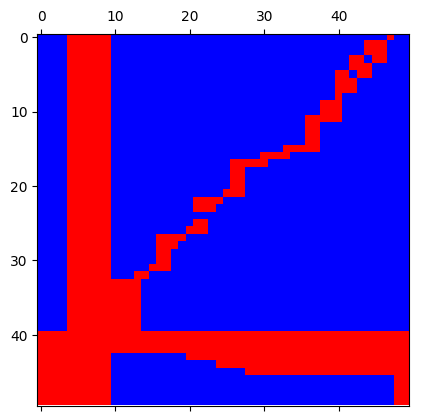
\includegraphics[width=1\linewidth]{images/assign2/visu_50-part1/t20}
      \caption{$t_{20}$}
      \label{fig:t20_50part1}
    \end{subfigure}
    \begin{subfigure}{.33\textwidth}
      \centering
      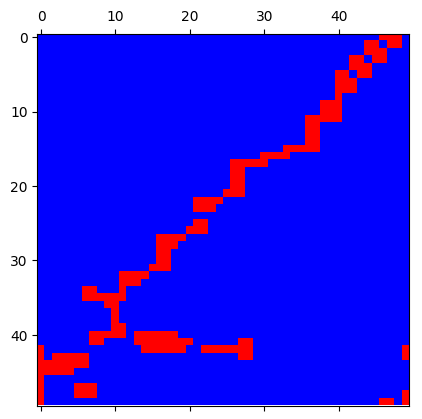
\includegraphics[width=1\linewidth]{images/assign2/visu_50-part1/t50}
      \caption{$t_{50}$}
      \label{fig:t50_50part1}
    \end{subfigure}
    \caption{Visualization of a the lattice with unconditional imitation,
    Moore neighborhood and weak prisoner's, dilemma}
    \label{fig:visu50part1}
\end{figure}

% Coop level for all others
\begin{figure}
    \begin{subfigure}{.5\textwidth}
        \centering
        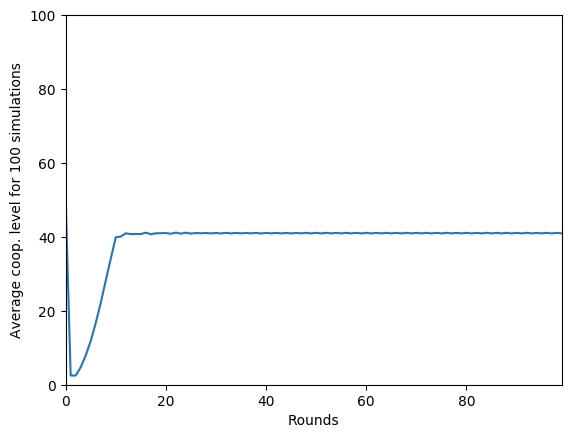
\includegraphics[width=1\linewidth]{images/assign2/20-part1}
        \caption{20x20}
        \label{fig:20moorepart1}
    \end{subfigure}
    \begin{subfigure}{.5\textwidth}
        \centering
        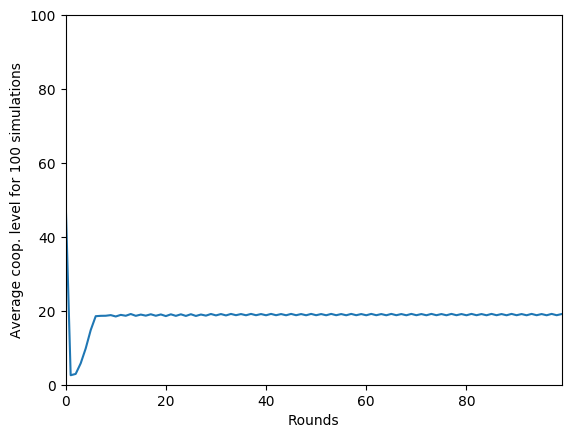
\includegraphics[width=1\linewidth]{images/assign2/12-part1}
        \caption{12x12}
        \label{fig:12moorepart1}
    \end{subfigure}
    \begin{subfigure}{.5\textwidth}
        \centering
        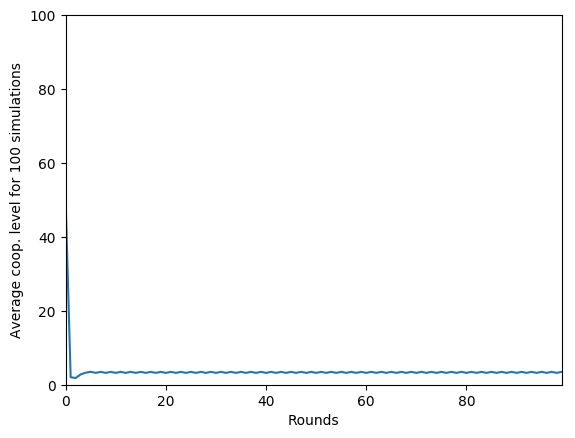
\includegraphics[width=1\linewidth]{images/assign2/8-part1}
        \caption{8x8}
        \label{fig:8moorepart1}
    \end{subfigure}
    \begin{subfigure}{.5\textwidth}
        \centering
        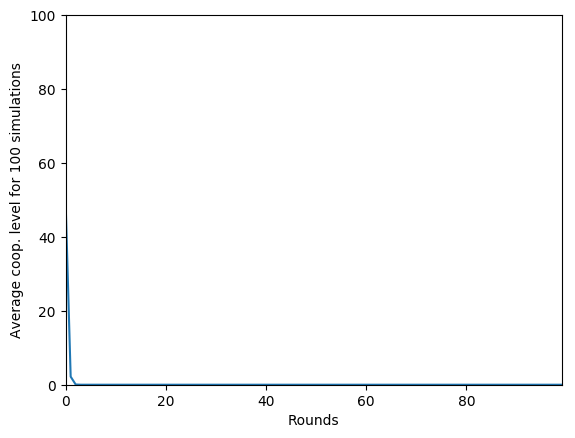
\includegraphics[width=1\linewidth]{images/assign2/4-part1}
        \caption{4x4}
        \label{fig:4moorepart1}
    \end{subfigure}
    \caption{Cooperation level using unconditional imitation, Moore neighborhood
    and weak prisoner's dilemma}
    \label{fig:otherpart1}
\end{figure}

\section{Part II}

\section{Update mechanism}

\begin{equation}
    P_{ij} = (1 + [W_j - W_i] / [N\cdot(max\{P, R, T, S\}
    - min\{P, R, T, S\}])/2
\end{equation}

\paragraph{Intuitive observation}

This probabilty is interesting to be used as an update mechanism because
the probability to change the action to the neighbor action is
proportional to the difference between the players payoffs.

\paragraph{Probability variables}

$[W_j - W_i]$ is the difference between the two payoffs.
$N$ represent the number
of neighbor that the payoff calculation are based on. The difference
between the maximum and minimum multiply by $N$ is
the maximum payoff of a player. Since the payoffs cannot be bigger than
the maximum score, it is clear that $P_{ij}$ is a probability.

\paragraph{Analysis}

We can highlight different result from
the fration
$[W_j - W_i] / [N\cdot(max\{P, R, T, S\}
- min\{P, R, T, S\}]$
between the difference of payoffs and the maximum score:

\begin{enumerate}
    \item Fraction is positive when $W_j > W_i$. A special
    case is when $W_j$ is maximum and $W_i$ is null, the fraction is equal to 1.
    \item Fraction is negative when $W_i > W_j$. A special
    case is when $W_i$ is maximum and $W_j$ is null, the fraction is equal to -1.
    \item Fraction is equal to 0 when $W_i = W_j$
\end{enumerate}

By using the full definition of the probablity we can see that when in
case (1), it is more probable that the player will change is action
to the neighbor action, and sure if the fraction is equal 1
because $P_{ij} = 1$. When in (2),
it is more probable that the player will keep is action, and sure that
he will not change it when the fraction is equal to -1
because $P_{ij} = 0$. When in (3),
$P_{ij} = \frac{1}{2}$,
the payoff of the player and his neighbor are the same, which means that
both of their actions lead to the same payoff, so the probability to change
or to keep is the same.

% Coop level for 50
\begin{figure}
    \begin{subfigure}{.5\textwidth}
        \centering
        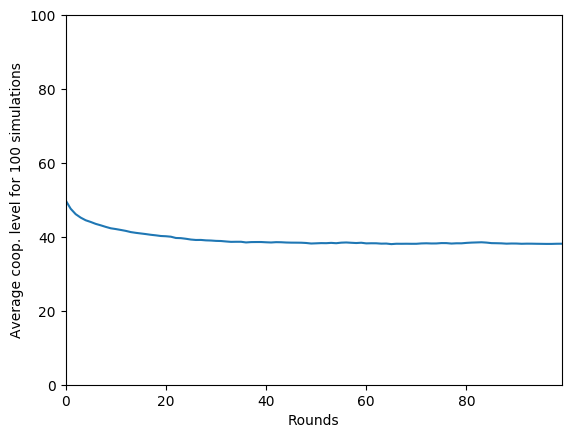
\includegraphics[width=1\linewidth]{images/assign2/50-part2}
        \caption{Moore neighborhood}
        \label{fig:50moorepart2}
    \end{subfigure}
    \begin{subfigure}{.5\textwidth}
        \centering
        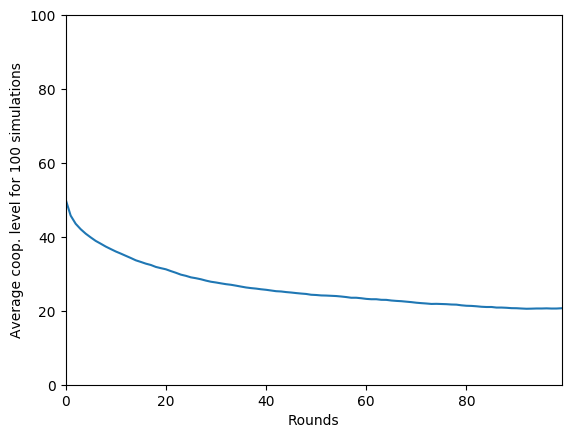
\includegraphics[width=1\linewidth]{images/assign2/50_vonneumann-part2}
        \caption{Von Neumann neigborhood}
        \label{fig:50vonpart2}
    \end{subfigure}
    \caption{Cooperation level using replicator rule and
    snowdrift game on a 50x50 lattice}
    \label{fig:50part2}
\end{figure}

% Visualization for 50
\begin{figure}
    \begin{subfigure}{.33\textwidth}
      \centering
      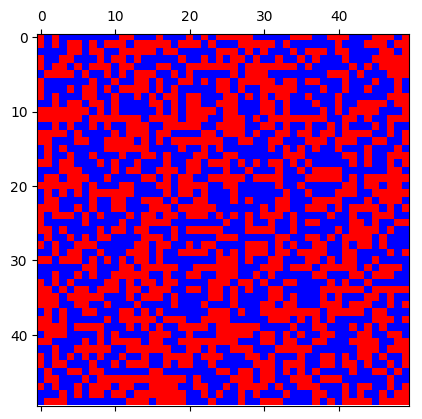
\includegraphics[width=1\linewidth]{images/assign2/visu_50-part2/t0}
      \caption{$t_0$}
      \label{fig:t0_50part2}
    \end{subfigure}
    \begin{subfigure}{.33\textwidth}
      \centering
      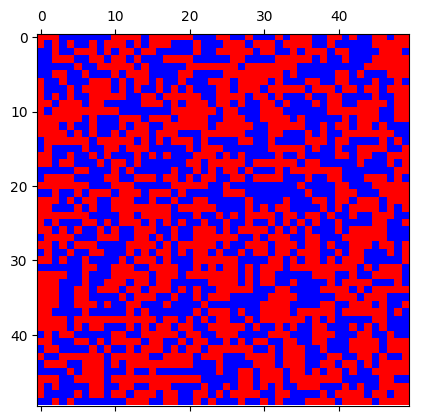
\includegraphics[width=1\linewidth]{images/assign2/visu_50-part2/t1}
      \caption{$t_1$}
      \label{fig:t1_50part2}
    \end{subfigure}
    \begin{subfigure}{.33\textwidth}
      \centering
      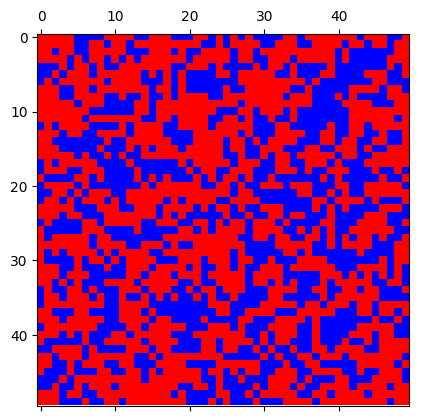
\includegraphics[width=1\linewidth]{images/assign2/visu_50-part2/t5}
      \caption{$t_5$}
      \label{fig:t5_50part2}
    \end{subfigure}
    \begin{subfigure}{.33\textwidth}
      \centering
      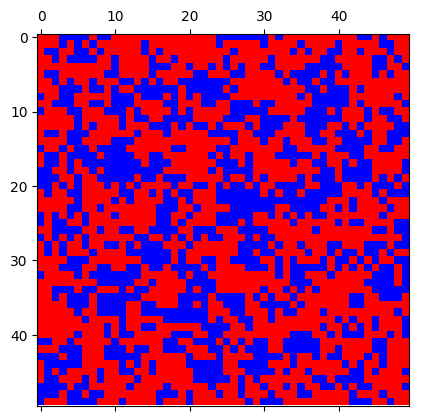
\includegraphics[width=1\linewidth]{images/assign2/visu_50-part2/t10}
      \caption{$t_{10}$}
      \label{fig:t10_50part2}
    \end{subfigure}
    \begin{subfigure}{.33\textwidth}
      \centering
      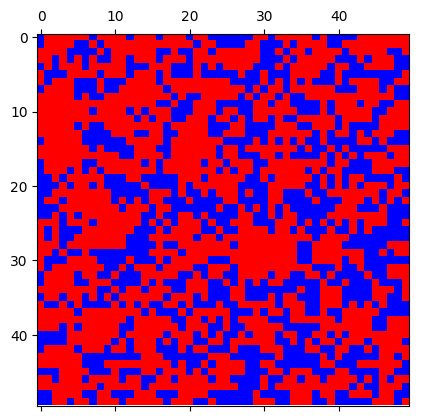
\includegraphics[width=1\linewidth]{images/assign2/visu_50-part2/t20}
      \caption{$t_{20}$}
      \label{fig:t20_50part2}
    \end{subfigure}
    \begin{subfigure}{.33\textwidth}
      \centering
      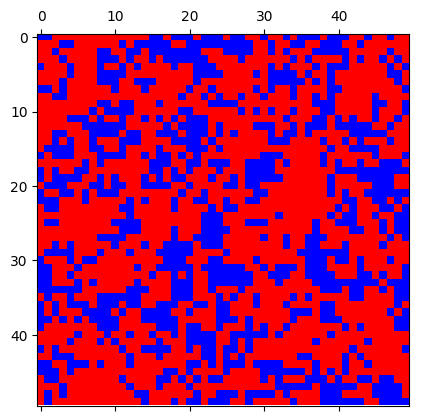
\includegraphics[width=1\linewidth]{images/assign2/visu_50-part2/t50}
      \caption{$t_{50}$}
      \label{fig:t50_50part2}
    \end{subfigure}
    \caption{Visualization of a the lattice with replicator rule,
    Moore neighborhood and snowdrift game}
    \label{fig:visu50part2}
\end{figure}

% Coop level for all others
\begin{figure}
    \begin{subfigure}{.5\textwidth}
        \centering
        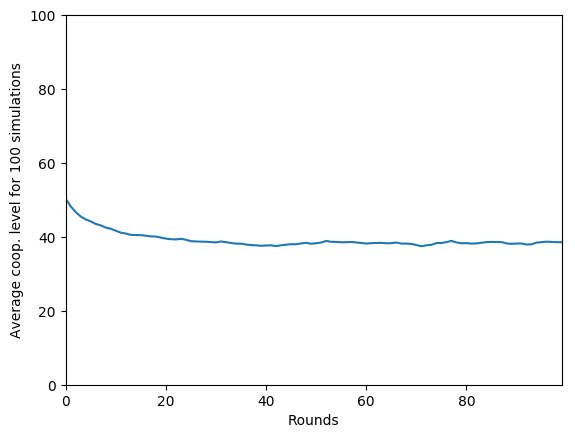
\includegraphics[width=1\linewidth]{images/assign2/20-part2}
        \caption{20x20}
        \label{fig:20moorepart2}
    \end{subfigure}
    \begin{subfigure}{.5\textwidth}
        \centering
        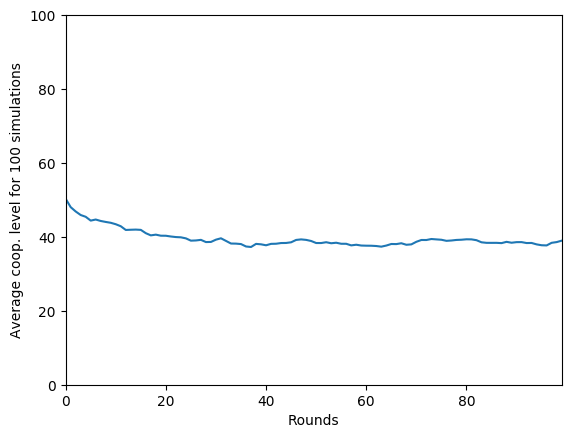
\includegraphics[width=1\linewidth]{images/assign2/12-part2}
        \caption{12x12}
        \label{fig:12moorepart2}
    \end{subfigure}
    \begin{subfigure}{.5\textwidth}
        \centering
        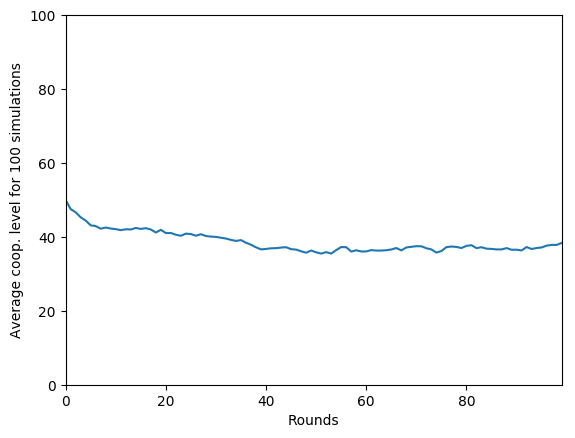
\includegraphics[width=1\linewidth]{images/assign2/8-part2}
        \caption{8x8}
        \label{fig:8moorepart2}
    \end{subfigure}
    \begin{subfigure}{.5\textwidth}
        \centering
        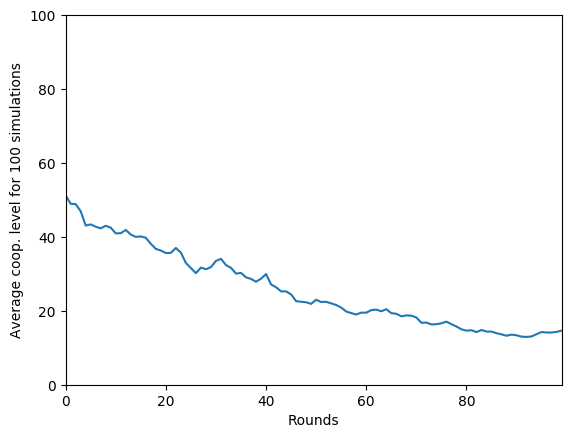
\includegraphics[width=1\linewidth]{images/assign2/4-part2}
        \caption{4x4}
        \label{fig:4moorepart2}
    \end{subfigure}
    \caption{Cooperation level using replicator rule, Moore neighborhood
    and snowdrift game}
    \label{fig:otherpart2}
\end{figure}


\end{document}
